\chapter{Curriculum Vit\ae}

\setcounter{secnumdepth}{0} % Suppress section numbering
\setlength\parindent{0pt} % Stop paragraph indentation

\vspace{-5mm}

\begin{minipage}{0.6\textwidth}
\section*{Personal information}
\cvline{Name}{Enrico Siragusa}
\cvline{Date of birth}{28 March 1985}
\cvline{Citizenship}{Italian}
\cvline{Address}{Meininger Str. 10}
\cvline{}{10823 Berlin, Germany}
\cvline{Mobile phone}{ +49 (0)160 5168591}
\cvline{Email address}{\href{mailto:enrico.siragusa@fu-berlin.de}{enrico.siragusa@fu-berlin.de}}
\end{minipage}%
\begin{minipage}{0.4\textwidth}
\vspace{5mm}
\flushright{\doublebox{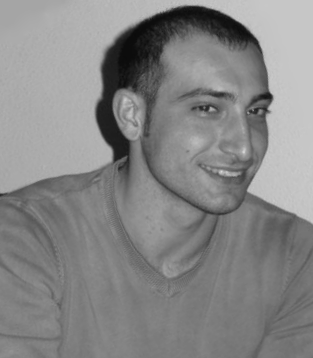
\includegraphics[height=100pt]{figures/enrico}}\hspace{1.5cm}}
\end{minipage}

\section*{Education}
\cventry{2010--now}{PhD in Bioinformatics}{Free University of Berlin}{IMPRS for Computational Biology and Scientific Computing}
\cventry{2008--2009}{MSc in Bioinformatics and Genome Research}{Bielefeld University}{EU exchange program}
\cventry{2007--2010}{MSc in Computer Science}{UMLV Paris-Est}{Mention {\guillemotleft}Bien{\guillemotright}}
\cventry{2006--2007}{BSc in Computer Science and Maths}{UMLV Paris-Est}{Degree achieved via the international project {\guillemotleft}Vinci{\guillemotright} sponsored by Italian and French Ministry of Education}
\cventry{2003--2006}{BSc in Computer Science}{Palermo University}{Grade {\guillemotleft}110/110 cum Laude{\guillemotright}}

\section*{Professional experience}
\cventry{2014--now}{Bioinformatics Researcher}{Berlin Institute of Health}{Berlin, Germany}
\cventry{Apr--Jul 2013}{CUDA Software Engineer}{NVIDIA Research}{Berlin, Germany}
%\cvline{}{\footnotesize I designed a novel technique for cross-architecture C\texttt{++} generic programming and applied it to accelerate the SeqAn library on the NVIDIA Tesla architecture. I implemented efficient approximate string matching algorithms on the FM-index.}
\cventry{2009--2010}{Software Developer}{EffiCity}{Paris, France}
%\cvline{}{\footnotesize Engineering and optimization of relational, non-relational, and geographical databases.}
\cventry{2007--2008}{Software Developer}{eoRezo}{Paris, France}
%\cvline{}{\footnotesize Development of high-performance web-services, web-caches, and messaging infrastructures.}

\section*{Teaching experience}
\cvline{WS 2011}{Data Structures and Algorithms for Bioinformatics --- practical lectures and lab. \textit{FU Berlin, 19700}.}
\cvline{SS 2010}{Project Management with SeqAn. \textit{FU Berlin, 19588a}.}

\section*{Summer schools}
\cvline{Aug 2013}{Otto Warburg Summer School on NGS and its Impact on Genetics.}
\cvline{Sep 2011}{Otto Warburg Summer School on Evolutionary Genomics.}

\section*{Technical skills}
\cvline{Languages}{\small C\texttt{++}, OpenMP, Python, Perl, R, Matlab, Java, JavaScript, Bash, \LaTeX, PGF/Ti\textit{k}Z.}
\cvline{Libraries}{\small STL, Boost, Thrust, NumPy, OpenCV, GTK\texttt{+}, Tk, Django, ExtJS, JQuery.}
\cvline{Tools}{\small Xcode \& Instruments, Eclipse, CMake, GNU Toolchain, Valgrind, Flex \& Bison, PerlXS, Subversion, Git, Mercurial.}
\cvline{Methods}{\small Generic Programming, Object Oriented Programming, Design Patterns.}
\cvline{Databases}{\small MySQL, PostgreSQL and PostGIS, MongoDB.}

\section*{Language skills}
\cvline{Italian}{Mother tongue}
\cvline{English}{Fluent}
\cvline{French}{Fluent}
\cvline{Spanisch}{Fluent}
\cvline{German}{Intermediate}

\section*{Transferable skills}
\subsection*{\emph{Workshops provided by the Dahlem Research School}}
\cvtext{Scientific writing in the life sciences. Teaching and learning at university level. Advanced scientific presentation. Confident speaking with impact. Speed reading.}

\section*{Presentations and talks}
\cvtext{Massively parallel methods for NGS read mapping. \emph{Otto Warburg Summer School 2013 on NGS and its Impact on Genetics.}}
\cvtext{CUDA-accelerated SeqAn: effective sequence analysis on GPUs. In \emph{GPU Acceleration of Bioinformatics Pipeline, NVIDIA Corporation, BoF Session.} \emph{ISMB/ECCB 2013.}}
\cvtext{Scalable string similarity search/join with approximate seeds and multiple backtracking. \emph{EDBT/ICDT 2013 Workshop on Scalable String Similarity Search/Join.}}

\section*{Publications}

%\bibliographystyle{natbib}

\cvtext{\bibentry{Siragusa2015b}}

\cvtext{\bibentry{Siragusa2015}}

\cvtext{\bibentry{Wandelt2014}}

\cvtext{\bibentry{Siragusa2013b}}

\cvtext{\bibentry{Siragusa2013}}

\cvtext{\bibentry{Giancarlo2007}}
